\section{Anforderungsanalyse}


\subsection{VJing}

Die Pr\"asentation von visuellem Material setzt gewisse Technik vorraus, welches verschiedene Medienformate unterst\"utzt,
andere nur unter Umst\"anden und manches vielleicht gar nicht. Beispielsweise unterst\"utzt ein Videorecorder keine digitalen
Videodateien. M\"ochte man die Performance mithilfe von Videoclips realisieren und braucht Funktionen wie Zeitraffer oder
automatisches Vorw\"arts-R\"uckw\"arts-Abspielen ist eine Software gesucht die das kann. Legt man viele Videos \"ubereinander 
setzt das gewisse Rechenressourcen vorraus, mit denen das Resultat dargestellt wird.

Vor allem auf der Softwareseite sind viele Abh\"angigkeiten zu beachten. Da bei dem VRC-Konzept das Abspielen von Videoclips
nicht verloren gehen soll, die Darstellung und Animation von 3D-Inhalten zu Musik prim\"ares Ziel sind, stellt sich die Frage
mit welche Libraries in Frage kommen.

Der Bedienbarkeit kommt auch ein eigenes Feld zu. Viele VJs benutzen MIDI Controller, um die Darstellung zu steuern, da 
Potentiometer gef\"uhlvolles Einstellen von Parametern erm\"oglicht. Gleichzeitig muss ein VJ auf drastische \"Anderungen 
an der Darstellung vorbereitet sein.

\subsubsection{Hardware und Software}

Die Hardware sollte mobil sein. Ein Videoprojektor und ein Laptop sind die Grundlage f\"ur das Performen. F\"ur die 
Soundanalyse kann man direkt das Signal von einem Verst\"arker abgreifen oder \"uber ein Mikrofon aufnehmen. Gleichzeitiges 
Abspielen von mehreren Visuals auf einmal sollte m\"oglich sein. Das Anordnen der Visuals in einem dreidimensionalen
Raum erfordert Software, die das kann und auf Hardwareseite ist 3D-Beschleunigung n\"otig. 
\\
Ein Laptop, der mehrere Videoclips und 3D-Modelle auf einmal berechnet und dazu den Sound analysiert und mit der Szenerie
verkn\"upft um Animationen und Visualit\"at zu erzeugen, braucht ein gewisses Mass an Rechenkraft. Da nicht nur die 
Grafikkarte zum Rendern beansprucht wird, sondern vor allem auch die CPU f\"ur das schnelle Analysieren des Sounds und 
Ausf\"uhren von Funktionen zust\"andig ist, darf hier nicht gespaart werden. Je nach dem wie Aufw\"andig die Szenerie
gestaltet ist ergeben sich Mengen von Polygonen, die transformiert werden m\"ussen. Auch hier sollten gen\"ugend 
Leistungsreserven vorhanden sein, weshalb von Integrierten Grafikkarten abzuraten ist, da dedizierte Grafikkarten 
momentan mehr Leistung haben.

Laptops, die f\"ur Computerspiele, technisches Zeichnen, Bilder- und Videoverarbeitung  konstruiert sind 
verf\"ugen meist schon \"uber eine dedizierte Grafikkarte und eine besserer CPU als regul\"arer B\"urorechner.
\\
Hinsichtlich Kosten und Plattformwahl soll m\"oglichst freie Software verwendet werden. Eine leicht erlernbare 
Programmiersprache zur Erstellung von Visuals soll es VJs mit mit geringen Programmierkenntnissen erm\"oglichen Visuals
f\"ur das Pr\"asentationsprogramm zu programmieren. Eine freie Grafikbibliothek wie OpenGL bietet eine Grundlage f\"ur 
Rendering der Szenerie, jedoch stellt das Programmieren von OpenGL eine gro\ss e H\"urde f\"ur VJs mit nicht so tiefen
Programmierkenntnissen dar. Deher muss es die Komplexit\"at von OpenGL vereinfacht werden und Bibliotheken die auf OpenGL
aufsetzen benutzt werden.


\subsubsection{Bedienbarkeit}

F\"ur die Bedienung sollen standard Eingabeger\"ate wie Tastatur und Maus gen\"ugen. Vor allem die Einstellung der Ansicht
und Positionierung der Visuals in einem 3D-Raum muss auf einer Tastatur komfortabel m\"oglich sein - und das 
wom\"oglich stundenlang. \"Uberblendungen und Visualwechsel beinhalten viele Aktionen wie das \"Andern von Transparenzen oder
Farben und muss fl\"ussig machbar sein. Die Ansicht durch eine virtuelle Kamera erfordert eine bewegliche Kamera. Bei 
Rotationen der Kamera ist es wichtig die Orientierung nicht zu verlieren.

Eine Kombination aus Spielsteuerung f\"ur das ansteuern der Visual-Objekte und der Kamera scheint mit einer Tastatur 
realisierbar und sinnvoll. Das Anzeigen und Einstellen von Statusinformationen von Kamera,
Soundanalyse und aktiven Visuals sowie die \"Ubersicht der verf\"ugbaren Visuals erfordert eine geeignete 
Benutzerschnittstelle mit Panelen an denen Parameter abgelesen und ge\"andert werden k\"onnen.

Wichtig ist eine Reservierung von Tasten auf der Tastatur  f\"ur die Steuerung der ins Visual individuell einprogrammierten
Routinen.


\subsection{Visuals}

In dem VJ-Konzept ist der Fokus auf eine liberale Visualgestaltung ausgerichtet. Operationen wie Verschieben, Skalieren, 
Rotieren und transformation zu Musik sollen jedem Visual aufgrund seines Charakters als Objekt in einem 3D-Raum m\"oglich sein. 
Der Sound
soll von Visuals genutzt werden k\"onnen um Effekte auszul\"osen oder zu beeinflussen. Visuals bestehen bspw aus Punkten die zu 
geometrischen Formen verbunden werden k\"onnen. Vorgefertigte 3D-Modelle sollen unterst\"utzt werden. Texturen k\"onnen 
aus Bilddateien, Shaderprogrammen oder Videoclips bestehen. Durch das Programmieren der Visuals hat man 
die M\"oglichkeit eigene Bibliotheken zu benutzen und Algorithmen zur Visualisierung zu implementieren. 
 
\subsubsection{Erstellen}

F\"ur das Erstellen von Visuals ist es wichtig, dass der K\"unstler seine Visualidee verwirklichen kann. G\"angige 
Formate f\"ur Bilddateien und Videos m\"ussen unterst\"utzt werden. Dadurch hat der (VJ)K\"unstler die M\"oglichkeit
verschiedene Tools zu benutzen um Bilder oder Videos zu pr\"aparieren. Im 3D-Raum k\"onnen diese dann als Texturen auf
Fl\"achen dargestellt werden. 

Vor allem soll aber der VJ auch Punkte zu Poligonnetzen verbinden k\"onnen. So k\"onnen 3D-Modelle mit 3D-Grafikprogrammen
wie bspw Blender erstellt und in Visuals verwendet werden. Dadurch ist es auch m\"oglich vorgefertigte 3D-Modelle aus dem
Internet zu benutzen, welche von Anbietern zum Beispiel f\"ur CAD (Computer Aided Design), oder Spiele zum Download bereitgestellt 
werden. Manche Formate bieten die M\"oglichkeit Animationen zu direkt im Model zu definieren. Unabh\"angig von Formaten
m\"ussen die Inhalte auch durch selbstgeschriebene Funktionen animierbar sein. 

Mit eigens definierten Funktionen kann man auf die Skalierung, Farbe, Transparenz oder Positionierung Einfluss nehmen.
Das Soundsignal als wichtiger Bestandteil muss in Funktionen verarbeitbar sein. Durch die Analyse des Soundsignals k\"onnen 
sich Funktionen dynamisch gegenseitig aufrufen und mit der k\"unstlerischen Intention verkn\"upft werden. So kann das 
Visual programmiert werden auf B\"asse vorprogrammierte Effekte auszul\"osen.

Mit der Programmierung der Tasteneingabe kann das Visual gesteuert werden. Die Zustandsa\"nderung auf eine Tasteneingabe
muss bei der Erstellung definiert werden k\"onnen. Auch hierbei sind Funktionen die Grundlage daf\"ur.

primitive, 3d meshes, 
fertige modelle mit blender
videoclips
tastenbelegung


\subsection{Darstellung}

Ein Programm zur Darstellung der Visuals ist n\"otig um alle Visuals mit dem Soundsignal zu versorgen, Eingaben entgegen
nimmt und auf Parameter der Visuals zugreiffen kann. 


Das Programm stellt den 3D-Raum bereit in denen die Visuals geladen werden k\"onnen sowie eine \"Ubersicht \"uber
Parameter, Eingaben und Metainformationen \"uber die Zust\"ande der Visuals. Eine \"Ubersicht \"uber die Positionen
der Visuals und Kameras sowie der Ausrichtung der Kamera hilft dabei Szenen und Kameraeinstellungen zu koordinieren.

Diese Anforderungen k\"onnen in einer GUI untergebracht werden. Eine GUI fasst dabei Eingabeschnittstellen f\"ur die Visuals,
die Kameras und Soundeinstellungen zusammen, an denen die wichtige Daten \"uber den Zustand des Dargestellten abgelesen
werden k\"onnen.

Eine Ansicht durch eine Kamera wird dabei in Vollbildschirmmodus an das Ausgabeger\"at (Videoprojektor) geschickt. Eine 
andere Ansicht in den Raum erm\"oglicht das direkte Interagieren mit Visuals und Kamera. Diese Ansicht soll den
Computerspielcharakter bereitstellten wodurch direkte Manipulation an Rotation und Position m\"oglich ist.

%Dabei m\"ussen verschiedene Tasks ausgef\"uhrt werden.
%programm zur das sound verarbeitet, 
%parameter einstellung
%taskmanager, 
%Eingabe verarbeiten

%\subsubsection{3D Raum und Camera}

%Durch die Ansicht des 3D-Raums durch die virtuelle Kamera wird der 3D-Raum zum Beh\"alter f\"ur Visuals, der betrachtet wird.
%Die Positionierung der Kamera und der Visuals

%container fuer visuals
%beinhaltet cameras zur ansicht
%Camerapositionierung

\subsubsection{Performen}

Die Performance des VJs besteht aus dem Laden und Entfernen von Visuals in dem 3D-Raum. Visuals werden um die
Kamera angeordnet und bilden die Szenerie. Bei \"Anderungen in der Musik wird die Szenerie angepasst oder der
Blickwinkel auf die Szenerie ge\"andert. 

Musik enth\"alt oft H\"ohepunkte und viele k\"unstlerische Stilmittel.
Anhand der akustischen Wahrnehmung des VJs kann an Wendepunten in der Musik in Echtzeit die Performance des VJs
an die Musik anpasst werden. Durch hineinfaden eines anderen Visuals, einem Schnitt oder dem Ausl\"osen eines 
Effekts erh\"alt die Musik ihre visuelle Individualit\"at w\"ahrend des Events.

Dabei soll das Programm Operationen wie Schnitte, Kamerafahrten, Positionierung und Rotationen, Fading oder
\"Anderungen an der Kameraeinstellung schnell auf Visual und Kamera f\"ur den VJ schell ausf\"uhrbar gestalten.
Hauptaugenmerk f\"ur das Performen ist die Usability. Da die Eingabeger\"ate f\"ur den Anfang aus 
Maus und Tastatur bestehen muss ein geeignetes Bedienkonzept erarbeitet werden.

\section{Entwurf}

Beim Entwurf m\"ussen \"Uberlegungen getroffen werden, welche die Auswahl der Software im Vorfeld auf
die in Frage kommenden Plattformen und n\"otige Programmbibliotheken reduziert. F\"ur die Implementierunge
wichtige Datenstrukturen m\"ussen so gew\"ahlt sein, dass man zur Laufzeit den Variablenzustand von Sound-
und Bedienungseingabe geschickt an allen relevanten Stellen abrufen und \"andern kann.

\begin{figure}[h!]
    \centering
    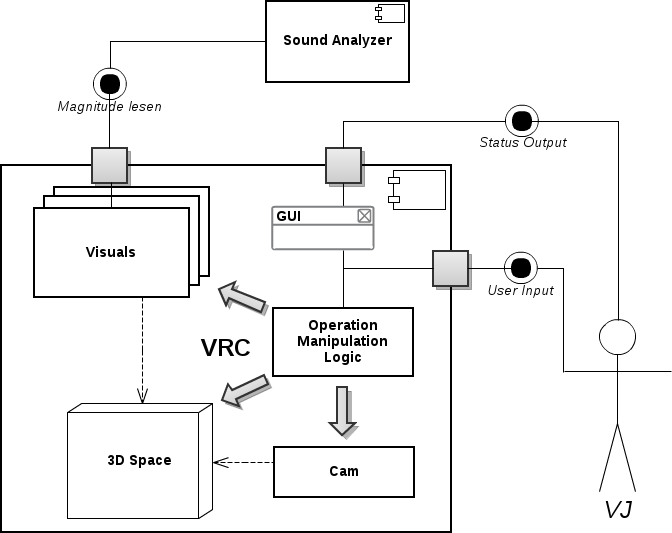
\includegraphics[width=1\textwidth]{pictures/vrc-component1.png}
    \caption{Strukturdarstellung des VJ-Konzeptprogramms VRC, bestehend aus Soundeingabe und einem Container f\"ur
    3D-Raum und Visuals welche von einem User f\"ur die VJ-Performance genutzt werden.}
\end{figure}

Das Konzept weist eine grundlegende Struktur aus 3D-Raum, Visuals, Soundeanalyse und Bedienkonzept auf


\subsection{\"Uberlegungen}

OpenGL entwickelte sich zum Industriestandard f\"ur interaktive 2D und 3D-Grafiken (* http://www.opengl.org/about/ )
und bietet eine umfangreiche Programmierschnittstelle f\"ur Grafikprogrammierung. Diese Schnittstelle wird durch
Grafikkarten hardwareseitig unterst\"utzt. F\"ur die meisten popul\"aren Sprachen gibt es Sprachanbindungen mit denen
man auf die Schnittstelle direkt zugreiffen kann. 

Spiel-Engines als Programmierger\"ust erscheinen vorteilhaft um 3D-Grafiken in Szene zu setzen. Durch die Beschr\"ankung
auf standard Eingabeget\"ate sind Spiel-Engines hervorragend f\"ur die Verarbeitung von Benutzereingabe und Steuerung
des 3D-Raums geeignet. Auch das Erstellen von Visuals erf\"ahrt durch die Verwendung von Spiel-Engines Vorteile. Elemente
werden in Visuals gruppiert und mit Funktionen unter Einbezug verschiedener Parameter modifiziert/transformiert. Anhand
des Soundsignals k\"onnen ausgew\"ahlte Parameter dem musikalischen Zufall \"uberlassen werden. Dadurch wird eine 
akustisch-visuelle Koppelung zwischen Visual und Umgebung m\"oglich. Die Soundeingabe soll m\"oglichst unabh\"angig von
technischen Faktoren m\"oglich sein. Laptops haben meist schon standardm\"a\ss{}ig ein Mikrofon eingebaut, das man als
standard Eingabeger\"at bei Performances nutzen kann. 

Wichtig vor allem ist, dass man Effekte durch Tastendruck ausl\"osen kann. Dazu m\"ussen Visuals frei programmierbar sein
um mit Code den Ablauf des Effekts zu definieren. Dadurch dass Tasten mit Programmierung belegt werden k\"onnen, sind f\"ur
die Visuals individuelle Funktionen programmierbar. Durch Anwendung der objektorientierten Programmierung k\"onnen 
Funktionen (Methoden) k\"onnen Objekte als Container f\"ur Funktionen und Daten dienen. Objektorientiertes Programmieren
eignet sich also f\"ur Visuals.


%OpenGL - Hardwarebeschleunigt
%Framework f\"ur OpenGL - Game Engine, SDL, Processing
%Mikrofon als Soundinput - standard laptops haben bereits mic
%Python/C++/Java - Comparision Libraries/Bindings
%Libraries - Soundanalyse, GUI, 
%Datenstrukturen f\"ur Visuals
%Visualrealisierung - OpenGL, eigene Funktionen

\subsubsection{Datenstrukturen}

Um die Visuals im Programm vorzuhalten und kann eine Liste mit Verweisen auf die Visuals verwendet werden. F\"ur 
die Visual-Elemente muss der 3D-Raum eine Datenstruktur vorhalten in den die Elemente hineingeladen werden k\"onnen.
Daf\"ur eignet sich eine Baumstruktur ganz gut. Der 3D-Raum stellt die Wurzel des Baums dar, jedes Visual ist ein
Kind des 3D-Raums. Ein Visual besteht aus einem Knoten, der als Wurzel f\"ur die Visual-Elemente fungiert
(siehe Abbildung). Dieser Baum stellt den Szenengraphen dar, in dem die OpenGL-Objekte der Visuals, wie Modelle, Texturen 
oder Videos geladen werden.

\begin{figure}[h!]
    \centering
    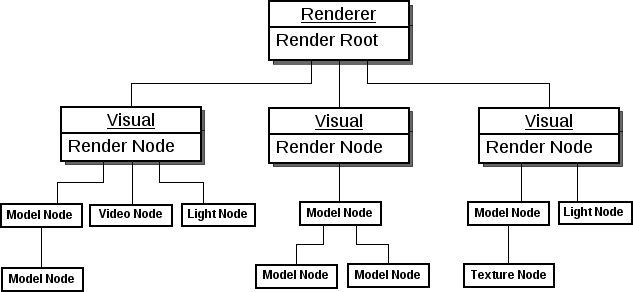
\includegraphics[width=1\textwidth]{pictures/data_structure1.png}
    \caption{Skizze eines Szenengraphen}
\end{figure}

%Liste mit VisualObjekt-Referenzen
%Visual-Elemente werden von Visuals in Graphen geladen
%VisualObjekt haelt Referenzen auf seine eigenen Elementobjekte im Graph der VisualElemente
%3D-Raum wird aufgebaut anhand des Graphen, der den zu sehenden Inhalt enth\"alt

\subsubsection{Soundanalyse}

Es gibt verschiedene M\"oglichkeiten Sound zu analysieren. Bei diesem Entwurf wird Wert darauf gelegt, dass 
Soundwerte auf einfache Art in den Visuals verarbeitet werden k\"onnen. Es sollen B\"asse, Mitten und H\"ohen
als Werte von  0 bis X abgelegt werden.

Die Soundanalysekomponente muss kontinuierlich die Soundeingabe verarbeiten. Das aufgenommene Frequenzband
wird unterteilt in Bassband, Mittelband und H\"ohenband. 
Das Bassband erstreckt sich \"uber die Frequenzen 0Hz bis 100Hz, die Mittelt\"one \"uber 100Hz bis 1000Hz,
und die Hoehen \"uber 1000Hz bis 44100Hz.
F\"ur jedes Band wird eine Magnitude berechnet, welche die Intensit\"at Samples auf den drei B\"andern angibt.
Dem Mikrofonsignal werden kontinuierlich Samples entnommen um die Magnitude \"uber den Frequenzb\"andern zu 
messen und in Soundzustandsvariablen zu speichern. Das Soundsignalsample ist ein Vektor aus 16Bit Integer-Werten -
f\"ur jede Frequenz ein Integer.

Eine einfache Methode den die Musik zu analysieren und einen Beat zu erkennen ist beispielsweise das Vergleichen
der Magnitude mit einem Grenzwert. Liegt die Magnitude \"uber dem Grenzwert, so kann das als Beat interpretiert
werden worauf eine Aktion folgen kann.

\subsubsection{Bedienung}

Da in den Anforderungen, die Benutzung von standard Eingabeger\"aten gefordert ist stellt vor allem die
Tastatur zur Steuerung von Visuals eine gute Plattform dar. Das Virtual Room Concept verh\"alt sich von der
Navigieren im 3D-Raum \"ahnlich dem des Bewegens von Aktoren in Computerspielen oder Arbeiten mit 3D-Programmen
wie Blender. In Computerspielen ist das was der Spieler sieht eine Ansicht einer virtuellen Kamera auf die ihn
virtuell umgebende Szenerie. Eine Grundlage zum Spielen ist das Bewegen des Agenten im Spiellevel, was dem 
Bewegen einer virtuellen Kamera in einem 3D-Raum entspricht.

Viele Spiele, allen voran First-Person-Spiele (FPS) haben oft f\"ur das Bewegen des virtuellen Agenten standardm\"a\ss{}ig
die selbe Tastenbelegung. Auch andere Funktionen wie die Auswahl von Gegenst\"anden ist oft \"ahnlich belegt.
Der gr\"o\ss{}te Unterschied zu den meisten FPS ist es wohl, dass man die Kamera, bzw die Visuals zus\"atzlich um die
L\"angsachse rotieren moechte.

In diesem Entwurf wird die Bedienung von FPS f\"ur die Kamera und Visuals adaptiert. F\"ur die Rotationen wird
auch die Tastatur verwendet. Hierf\"ur werden zus\"atzlich Belegungen definiert. Diese unterscheiden sich von
denen in FPS. In FPS wird f\"ur die den Nick- und Gier-Winkel h\"aufig die Maus verwendet. Da f\"ur Kamera und
Visual jeweils Rotationen und Bewegungen m\"oglich sein sollen, wird die Bedienung f\"ur diese Aktionen 
vereinfacht indem die selbe Belegung f\"ur Visual und Kamera gilt.

Die Abbildung zeigt den Entwurf f\"ur eine m\"ogliche Tastenbelegung.

\begin{figure}[h!]
    \centering
    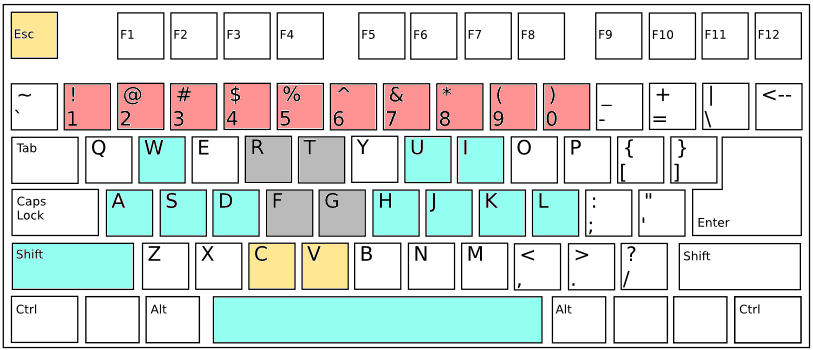
\includegraphics[width=1\textwidth]{pictures/usage_keyboard_layout1.png}
    \caption{Skizze eines Szenengraphen}
\end{figure}

F\"ur das Navigieren in der grafischen Oberfl\"ache wird die Maus verwendet.

%Tastatur, Maus
%Belegung Feste und programmierbare
%Bild

\subsubsection{Grafischen Oberfl\"ache}

In der grafischen Oberfl\"ache werden Daten aus dem Zustand des VRC aufbereitet, um Statusinformationen \"uber die
Visuals und Kamera anzuzeigen. Ausserdem werden \"uber die grafische Oberfl\"ache die Visuals in den 3D-Raum hinzugef\"ugt
oder entfernt. Wichtige gemeinsame Funktionen der Visuals k\"onnen in der grafische Oberfl\"ache zusammengefasst und 
der Manipulation zug\"anglich gemacht werden. 

Es m\"ussen die wichtigen Entit\"aten zum VJing schnell abrufbar sein. Gleichzeitig hat man aber nur begrenzten Platz auf
dem Bildschirm um Vorschaufenster und Menus unterzubringen.
Durch eine geschickte Unterbringung der Entit\"aten in Menus die mit Reitern navigierbar gestaltet sind, kann man Menuelemente
f\"ur den Visualpool, geladene Visuals, Kamera- und Soundeinstellungen gruppieren.
%Eine geschickte Unterbringung der Entit\"aten unter Reitern
%kann man seperat Visualpool, geladene Visuals, Kamera- und Soundeinstellungen erm\"oglicht das Gruppieren der verschiedenen
%Oberfl\"achenelemente. 
Die verschiedenen Entit\"aten Sound, Visuals und Kamera haben auch ihre eigenen Anforderungen an
Schnittstellen. So haben Visuals eine Schnittstelle f\"ur Skalierung, Transparenz, die Kamera aber nicht. Da es sich um
eine \"uberschaubare Menge an Entit\"aten handelt ist ein Reiterlayout f\"ur den VJ beim VJing ausreichend um Kontrolle
\"uber die Visualwerte zu behalten.

\begin{figure}[h!]
    \centering
    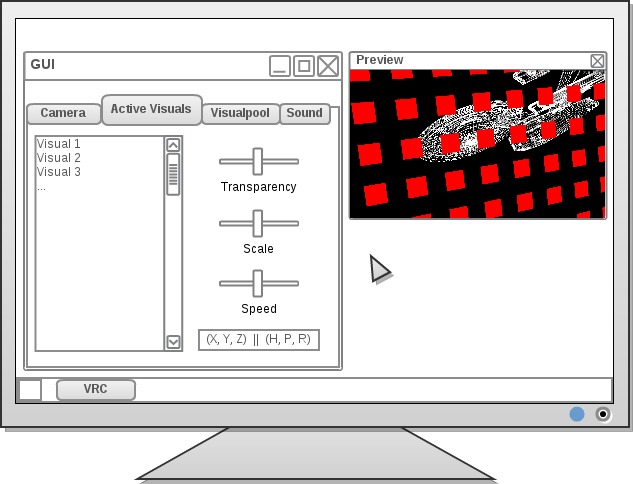
\includegraphics[width=1\textwidth]{pictures/gui1.png}
    \caption{Skizze der Grafischen Oberfl\"ache auf einem Monitor als Fenster f\"ur das Virtual Room Concept und die Vorschau}
\end{figure}


%\subsection{Spiele-Engine}

%Panda3d
%3d-Raum
%Kamera (eigene subsubsection)

\subsubsection{Szenengraph}

Renderer

\subsection{Visual-Klasse}

\subsubsection{Attribute}

\subsubsection{Methoden}



\section{Prototyp}

\subsection{Softwarewahl}

\subsection{Datenstruktur}

\subsection{Arbeitsweise}



\section{Test}

\section{Evaluierung}

\section{Verbesserungen}

\section{Resultat}
